\documentclass[titlepage]{article}
\usepackage{listings}
\usepackage{hyperref}
\usepackage{graphicx}

\lstset{basicstyle=\footnotesize\ttfamily,breaklines=true}

\usepackage{tikz}
\usetikzlibrary{arrows}

\begin{document}
\title{Trains Control 1}
\author{Justin McGirr (\#20413625), Peter Raboud (\#20437716)}
\maketitle

\section{Instructions}
\input{"README.tex"}

\section{Design Decisions}
% trainsrv
% - landmark + dead reckoning
% - basic sensor attribution
% - traversal of track, helper methods
% train alert srv
\subsection{Overview}

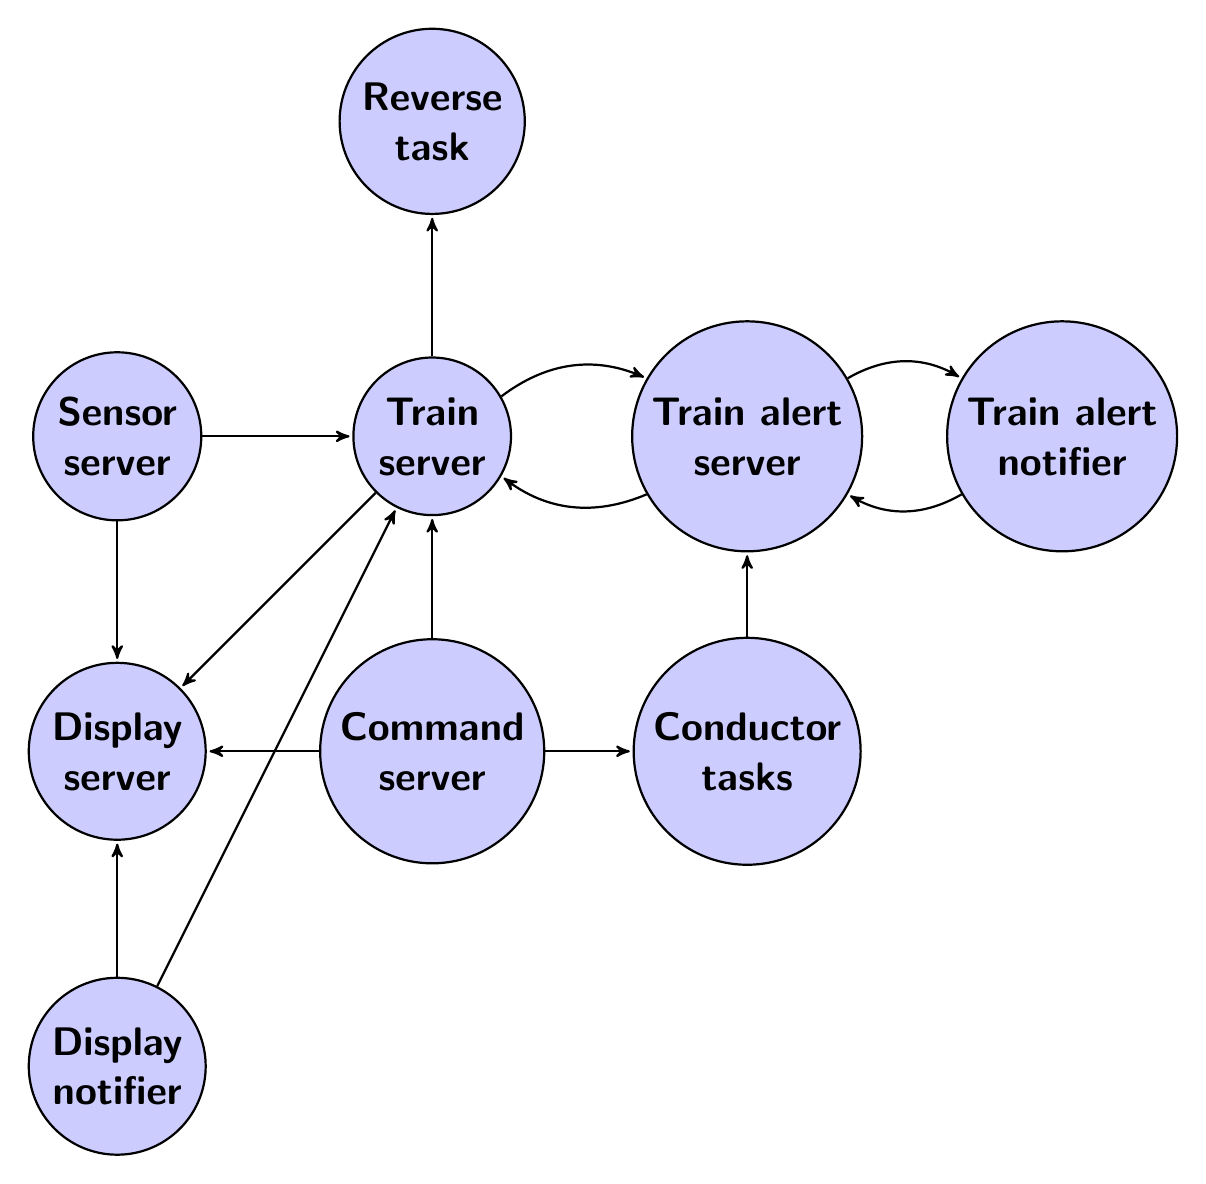
\begin{tikzpicture}[->,>=stealth',shorten >=1pt,auto,node distance=4cm,
  thick,main node/.style={circle,fill=blue!20,draw,font=\sffamily\Large\bfseries}]

  \node[main node] (d) [align=center]{Display \\ server};
  \node[main node] (dn) [align=center, below of=d]{Display \\ notifier};
  \node[main node] (c) [align=center, right of=d] {Command \\ server};
  \node[main node] (t) [align=center, above of=c] {Train \\ server};
  \node[main node] (ta) [align=center, right of=t] {Train alert \\ server};
  \node[main node] (r) [align=center, above of=t] {Reverse \\ task};
  \node[main node] (tan) [align=center, right of=ta] {Train alert \\ notifier};
  \node[main node] (s) [align=center, left of=t] {Sensor \\ server};
  \node[main node] (e) [align=center, right of=c] {Conductor \\ tasks};

  \path[every node/.style={font=\sffamily\small}]
    (dn) edge node {} (d)
         edge node {} (t)
    (t) edge [bend left] node {} (ta)
        edge node {} (d)
        edge node {} (r)
    (ta) edge [bend left] node {} (t)
         edge [bend left] node {} (tan)
    (tan) edge [bend left] node {} (ta)
    (c) edge node {} (t)
        edge node {} (d)
        edge node {} (e)
    (e) edge node {} (ta)
    (s) edge node {} (t)
        edge node {} (d)
    ;
\end{tikzpicture}

The cyclical dependency between the train alert server and train alert notifier
isn't a problem, since the server sends only once to set pass in parameters, and
the notifier is guaranteed to be receiving at that time.

The cyclical dependency between the train server and train alert server will
eventually be a problem, but we currently don't generate data rapidly enough for
this to cause problems.

We chose the following priorities for the tasks, in decreasing order:

\begin{enumerate}
\item Clock server notifier
\item Clock server
\item IO server notifier
\item IO server
\item Nameserver
\item Sensor server
\item Command server \& conductor tasks
\item Train alert notifier
\item Train alert server
\item Train server \& reverse tasks \& display notifier
\item Display server
\end{enumerate}

These are chosen to attempt to prioritize a response to inbound events from
the outside world.
However, these choices were made fairly naively.
Since we haven't had any problems which seem to originate from the chosen
priorities, we have spent little time trying to pick optimal priorities.

\subsection{Train Server}
To help manage the position of the trains, we changed the structure of the
tasks somewhat.
The train server was significantly altered.
Its original purpose was to be a simple server to interact with the track,
and was only a separate task so that we could globally keep track of the
speed a train is travelling at, and the orientation of the switches.

Now, this role has been significantly expanded into keeping track of the
positions of the trains, and inferring them based on incoming sensor data.
The train server keeps track of the last sensor a particular train hit.
Currently, we don't have proper sensor attribution, so we can only support
one train on track at once, but most of the train server is not written with
this assumption.
Since it's assumed that there is only one train on the track, and that
it is responsible for any sensor that is tripped.
Whenever a sensor is tripped, the assumed position of the train snaps to that
location.
This does not account for spurious sensor reads, other than ignoring
sensors that are continuously tripped.
(This was done since the sensor data from track B would otherwise be unusable.)

We infer the velocity of the train from these sensor reads, since we can
find the distance between this sensor, and the last one, and the time between
the reads, and calculate the velocity the train must have been travelling at.
This assumes that the train travels at a constant speed, which is acceptably
close to the truth for our purposes.
If the new sensor read means that the train seems to have travelled past
another sensor without tripping it, we are tolerant of this.
The distance travelled is considered to be the sum of the lengths of track
between each pair of sensors.
If more than one sensor would have needed to be missed, we still consider the
train to now be at this location, but we don't use this data to estimate
a velocity, since it's likely that something strange happened, and that
the data is not valid.
We incorporate the calculated velocity from each interval of track by computing
a new estimate of the velocity from the old estimate $v_e$, and the measured
velocity $v_a$.
We use the heurestic $v_e' = (1 - \alpha) v_e + \alpha v_a$, for $\alpha = 0.1$.

We also record how far off our previous estimate was, by computing where
we thought the train was at the moment that it tripped the sensor.
This discrepancy is displayed on the screen, and can be used as a measure of
how well-calibrated the train is.

Based on the estimated velocity, last sensor tripped, and time the last sensor
was tripped, we can estimate the current position of the train.
We also have the notion of "reanchoring" the trains - updating the last
known position to the currently estimated position.
Whenever we change the speed of a train, we reanchor that train.
When the orientation of a turnout is changed, we reanchor all trains.
This simplifies the computation that needs to be done to project the position
of the train, since it allows us to assume that the speed of the train and
orientation of the turnouts hasn't changed during the period we want to predict
the motion of the train.
By making these assumptions, as well as the assumption that the trains accelerate
instantaenously, we can calculate the distance traveled since the last position
a train was anchored at as simply the velocity of that train multiplied by
the elapsed time.

\subsection{Train alert server}
An operation that turns out to be useful when writing high-level train control
routines is to wait until the train is at a particular position.
We therefore created a train alert server to allow tasks to wait until a train
has arrived at a particular position.
The interface for the train alert server is
\texttt{int train\_alert\_at(int train\_id, struct position position)}.
The call blocks until the given train is estimated to have passed that position
on the track.
The function returns with the time at which the train passed that position
(time is measured in ticks since the startup of the clockserver).

The train server pushes notifications to the train alert server when
it detects that a train has hit a sensor.
The train alert server has a list of tasks which are waiting on a train
to be in a particular position.
If the sensor data tells the train alert server that this is the last
sensor the train will hit before arriving at the point of interest,
it starts a timer.
This timer waits for the estimated amount of time needed for the train
to travel to the POI, given it's current velocity and the orientation
of the turnouts.
It then wakes up, and signals the alert server that the waiting task can
now be woken up.

If the speed of the train or the orientation of the turnouts is changed
during this wait time, this needs to be detected.
Each await request maintains a nonce.
When a timeout is started, the worker task doing the timeout is given
that nonce.
If the orientation of the turnouts or speed of the train is changed,
the nonce is incremented by one, and a new timeout is begun.
If the nonce doesn't match the nonce that the timeout has, then something
must have changed during the timeout, so the timeout is simply ignored.

% TODO: Talk about cyclic dependency and why it's not currently a problem.

% acceleration profile
% initial v0 -> v1 way to get stopping distance (failed because can't run the
% train at low speed)
% partial deceleration method
% train selfie data, and conclusions
% bisection to find the stopping distance

% talk about nested functions?
% talk about new compiler?
\section{Acceleration/Stopping Distance Calibration}
One of the significant tasks in this deliverable was to calibrate the trains.
Above, we discuss the techniques used to calibrate the train's velocity,
including doing online calibration. In this section, we describe the various
techniques we attempted in order to calibrate the train
acceleration/deacceleration curve and stopping distance. This turns out to be
considerably more complex in general than measuring velocity, because getting
an accurate picture requires a significantly higher resolution than the sensors
normally provide, and there is no way to use sensors to measure the position of
a train which is currently stopped.

\subsection{Just Measure It}
We avoided using the simple "stop the train
at a sensor and measure displacement from the sensor" technique for quite a
while, under the justification that:
\begin{enumerate}
\item It is not a good way to get an estimate for the train position during
	the middle of the acceleration/deacceleration, and
\item There is no way to automate the data collection, so a distance (and
confidence interval) must be measured manually for each train at each possible
speed for a complete model. This takes hours, and is prey to human error.
\end{enumerate}
Even with complete measurements, and assuming the humans doing the measurements
are perfect (we try ;)), it is still difficult to refine the model with other
data that we have. For example, if we know that the train has not finished
accelerating, and hence is between two speeeds, what stopping distance do we
assume? If we know a particular section of track causes the trains to slow
down 10\%, how do we refine our estimate of stopping distance for that section
of track? The brute force model seemed like it could be subject to
combinatorial explosion in this case.

\subsection{Measure Part of it, Extrapolate}
After discussing the shortcomings of the "Just Measure It" approach, we decided
to adopt a different technique. Rather than measure the distance to stop
completely, we decided to just measure the time taken to travel a certain
distance while deaccelerating, and then extrapolate the actual stopping distance
based on our knowledge of the underlying deacceleration model in the train
(i.e. a quartic model). We spent a couple days on this, deriving the various
forms on the model, gathering measurements, testing our assumptions, and
refining bugs in the model (i.e. accounting for the delay between knowing that
a sensor tripped, and responding to the tripped sensor). However, we couldn't
get any better than about 30cm of accuracy with this model, and we started to
suspect that our model might not be accurate enough to be used in this way. As
part of an investigation on this front, we tried to come up with some techniques
for measuring what the actual deacceleration curve looked like.

\subsection{The Way You Stop}
After our extrapolation wasn't working, we wanted to come up with a way to
validate the underlying model we were assuming for the deacceration of the
train. We considered various techinques, but ultimately ended up using a
camera, suspended above the track, with a easily distinguishable color marked
on it for easy computerized tracking. We then captured data of the train
starting, stopping, starting, stopping, several times over, and extracted
the motion of the train by computing the centroid of the pixels which were
close to the easily distinguishable color in value. We then took the pairwise
differences of these points to get an approximation of velocity, smoothed the
curve to reduce image capturing noise, and tried to fit a curve. The resulting
curve would be well described as "definately not quartic nor cubic".
\begin{figure}[ht!]
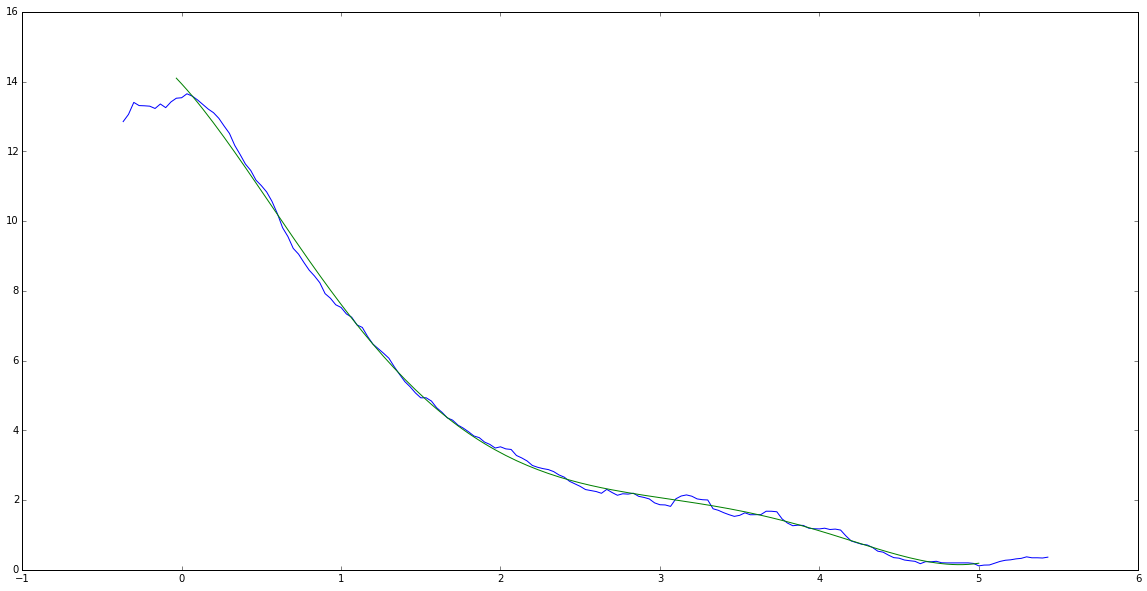
\includegraphics[width=\linewidth]{deaccel.png}
\caption{A fifth-order polynomial fit to experimentally derived data. Although
the fifth-order polynomial fits reasonably well, one can see the data is
definately not quartic nor cubic.}
\end{figure}
\begin{figure}[ht!]
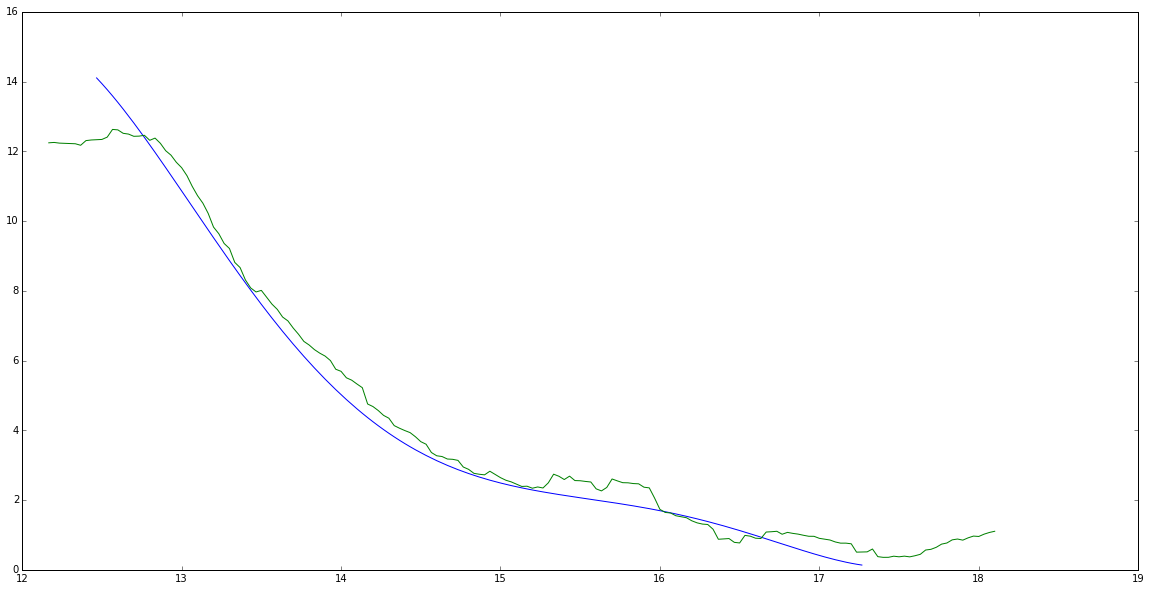
\includegraphics[width=\linewidth]{deaccel2.png}
\caption{The same polynomial that was fit to the previous set of deacceration
data seems to generalize fairly easily to other decceration curves from the
same speed, although some error is clearly present. The exact degree of error
is difficult to acertain, as there is still a fair bit of noise in the data
despite smoothing.}
\end{figure}
The apparatus used to enable this has been dubbed "the
train selfie stick".

\subsection{Bisecting for the stopping distance}
We wanted to find some way of automating collection of the stopping distance,
because collecting stopping distances with a tape measure, and hardcoding
them into a table is time consuming.
We originally wanted to derive the stopping distance from the acceleration curve,
but we had problems finding the acceleration curve, as described above.

A simpler technique turned out to be to start with a range of possible
values for the stopping distance, and then tighten this range by bisecting
the range iteratively.
At each step, we assume the stopping distance is the midpoint of
the range, and attempt to stop exactly on top of a sensor.
If the sensor is tripped, then we know that the actual stopping distance
is less than the estimate.
Otherwise, the actual stopping distance is greater.
Based on this knowledge, we can shrink the size of the feasible range by
one half.
We can then repeat this process until the interval is suitably small.

One problem that we have with this technique is that it assumes that results
are repeatable.
The train's stopping distance has a small amount of variance.
Also, the actual position of the train on the track when we tell it to stopping
is estimated.
This error causes the train to overshoot or undershoot the target sensor when
the train, on average, doesn't do this.
This causes the real stopping distance to be pruned out of the search range, so
the algorithm will never find the right result.

In particular, a flow in the way that velocity is estimated aggravated this problem.
We paused in the middle of the run, but the code that estimated the velocity
of the train assumed that we operated at a constant speed.
When the train accelerates, it moves at a small fraction of the top speed,
but the sensor data was interpreted to mean that the train's top speed is
very slow.
This introduced large errors in the velocity estimate for the train, which
caused the position estimated to be incorrect, which caused the problems described
above.
This could cause substantial error to be introduced into the final result, on
the scale of 10-20cm.
We fixed this problem by ignoring new velocity data soon after changing
the speed of the train.
An intelligent way to do this would be to know how long the train
takes to accelerate, but we don't know this precisely.
We instead make an intentionally high estimate of 4 seconds, to ensure
that the train will have finished accelerating after the timeout period.


\section{Source Code}
The source code is hosted on git, at \url{git.uwaterloo.ca/pgraboud/cs452-kernel}.
The version we wish to submit is the \texttt{tc1} tag, specifically
the commit:
\input{|"git rev-parse tc1 | ./../verbatim"}
\end{document}
